\section{Theory (50pt)}

To answer questions in this part, you need some basic knowledge of linear algebra and matrix calculus. Also, you need to follow the instructions:
\begin{enumerate}
\item Every vector is treated as column vector.
\item You need to use the numerator-layout notation for matrix calculus. Please refer to  \href{https://en.wikipedia.org/wiki/Matrix_calculus#Numerator-layout_notation}{Wikipedia} about the notation.
\item You are only allowed to use vector and matrix.
You cannot use tensor in any of your answer.
\item Missing transpose are considered as wrong answer.
\end{enumerate}

\subsection{Two-Layer Neural Nets}


You are given the following neural net architecture:
%
\[
\texttt{Linear}_1 \to f \to \texttt{Linear}_2 \to g
\]
%
where $\texttt{Linear}_i (x) = \bm{W}^{(i)}\bm x + \bm b^{(i)}$ is the $i$-th affine transformation, and $f, g$ are element-wise nonlinear activation functions.
When an input $\bm x \in \R^n$ is fed to the network, $ \bm {\hat{y}} \in \R^K$ is obtained as the output.

\subsection{Regression Task}
We would like to perform regression task.
We choose $f(\cdot) = (\cdot)^+ = \texttt{ReLU}(\cdot)$ and $g$ to be the identity function.
To train this network, we choose MSE loss function $\ell_\text{MSE}(\bm{\hat{y}}, \bm{y}) = \| \bm{\hat{y}} - \bm{y} \|^2$, where $y$ is the target output.

\begin{enumerate}[(a)]
\item
(1pt) Name and mathematically describe the 5 programming steps you would take to train this model with \texttt{PyTorch} using SGD on a single batch of data.

\item
(5pt) For a single data point $(x, y)$, write down all inputs and outputs for forward pass of each layer. You can only use variable $ \bm{x}, \bm{y}, \bm{W}^{(1)}, \bm{b}^{(1)}, \bm{W}^{(2)}, \bm{b}^{(2)}$ in your answer. (note that $\texttt{Linear}_i (\bm{x}) = \bm{W}^{(i)}\bm{x} + \bm{b}^{(i)}$).


\begin{center}
\begin{tabular}{ |c |c |c | }
\hline
Layer & Input & Output \\
\hline
$\texttt{Linear}_1$ &  &  \\
\hline
$f$ &  &  \\  
\hline
$\texttt{Linear}_2$ & &  \\
\hline
$g$ &  &  \\
\hline
\texttt{Loss} &  &  \\
\hline
\end{tabular}
\end{center}


\item
(8pt) Write down the gradient calculated from the backward pass. You can only use the following variables: $\bm{x}, \bm{y}, \bm{W}^{(1)}, \bm{b}^{(1)}, \bm{W}^{(2)}, \bm{b}^{(2)}, \frac{\partial \ell}{\partial \bm{\hat y}}, \frac{\partial \bm{z}_2}{\partial \bm{z}_1}, \frac{\partial \bm{\hat y}}{\partial \bm{z_3}}$ in your answer, where $\bm{z}_1, \bm{z}_2, \bm{z}_3, \bm{\hat y}$ are the outputs of $\texttt{Linear}_1, f, \texttt{Linear}_2, g$.

\begin{center}
\begin{tabular}{ |c |c | }
\hline
Parameter &  Gradient \\
\hline
$W^{(1)}$ &\\
\hline
$b^{(1)}$ &  \\ 
\hline
$W^{(2)}$ &  \\
\hline
$b^{(2)}$ & \\
\hline
\end{tabular}
\end{center}

\item 
(3pt) Show us the elements of $\frac{\partial \bm{z_2}}{\partial \bm{z_1}}$, $\frac{\partial \bm{\hat y}}{\partial \bm{z_3}}$ and $\frac{\partial \ell}{\partial \bm{\hat y}}$ (be careful about the dimensionality)?

\end{enumerate}


\textbf{Solution:}

(a)
\begin{enumerate}
\item Clear the gradients of all parameters. (model.zero\_grad())
\item Forward the Data (output = model.forward(batch))
\item Compute the loss function (loss = criterion(output, target))
\item Backpropagation to compute the gradients of the loss function with respect to the parameters. (loss.backward())
\item Update the parameters and update the optimizer status. (optimizer.step())
\end{enumerate}


(b)

$ \bm{x}, \bm{y}, \bm{W}^{(1)}, \bm{b}^{(1)}, \bm{W}^{(2)}, \bm{b}^{(2)}$

For a single data point $(x, y)$, we have:

\begin{center}
    \begin{tabular}{ |c |c |c | }
    \hline
    Layer & Input & Output \\
    \hline
    $\texttt{Linear}_1$ & $\bm{x}$ & $\bm{W}^{(1)}\bm{x} + \bm{b}^{(1)}$ \\
    \hline
    $f$ & $\bm{W}^{(1)}\bm{x} + \bm{b}^{(1)}$ & $f(\bm{W}^{(1)}\bm{x} + \bm{b}^{(1)})$ \\  
    \hline
    $\texttt{Linear}_2$ & $f(\bm{W}^{(1)}\bm{x} + \bm{b}^{(1)})$ & $\bm{W}^{(2)}f(\bm{W}^{(1)}\bm{x} + \bm{b}^{(1)}) + \bm{b}^{(2)}$ \\
    \hline
    $g$ & $\bm{W}^{(2)}f(\bm{W}^{(1)}\bm{x} + \bm{b}^{(1)}) + \bm{b}^{(2)}$ & $\bm{W}^{(2)}f(\bm{W}^{(1)}\bm{x} + \bm{b}^{(1)}) + \bm{b}^{(2)}$ \\
    \hline
    \texttt{Loss} & $\bm{W}^{(2)}f(\bm{W}^{(1)}\bm{x} + \bm{b}^{(1)}) + \bm{b}^{(2)}$  & $\| \bm{W}^{(2)}f(\bm{W}^{(1)}\bm{x} + \bm{b}^{(1)}) + \bm{b}^{(2)}  - \bm{y} \|^2$ \\
    \hline
    \end{tabular}
\end{center}


(c)


\begin{center}
    \begin{tabular}{ |c |c | }
    \hline
    Parameter &  Gradient \\
    \hline
    $W^{(1)}$ &\\
    \hline
    $b^{(1)}$ &  \\ 
    \hline
    $W^{(2)}$ & $2(\bm{W}^{(2)}f(\bm{W}^{(1)}\bm{x} + \bm{b}^{(1)}) + \bm{b}^{(2)}  - \bm{y}) f(\bm{W}^{(1)}\bm{x} + \bm{b}^{(1)})$  \\
    \hline
    $b^{(2)}$ & \\
    \hline
    \end{tabular}
\end{center}

(d)



\subsection{Classification Task}
We would like to perform multi-class classification task, so we set both $f, g = \sigma$, the logistic sigmoid function $\sigma(z) \doteq (1 + \exp(-z))^{-1}$.

\begin{enumerate}[(a)] 
\item
(2pt + 6pt + 2pt) If you want to train this network, what do you need to change in the equations of (b), (c) and (d), assuming we are using the same MSE loss function.

\item
(2pt + 6pt + 2pt) Now you think you can do a better job by using a \emph{Binary Cross Entropy} (BCE) loss function $\ell_\text{BCE}(\bm{\hat{y}}, \bm{y}) = \frac{1}{K}\sum_{i=1}^K -\big[y_i \log(\hat{y}_i) + (1 - y_i)\log(1 - \hat{y}_i)\big]$.
What do you need to change in the equations of (b), (c) and (d)?

\item
(1pt) Things are getting better.
You realize that not all intermediate hidden activations need to be binary (or soft version of binary).
You decide to use $f(\cdot) = (\cdot)^+$ but keep $g$ as $\sigma$. Explain why this choice of $f$ can be beneficial for training a (deeper) network.


\end{enumerate}

\textbf{Solution:}
(a)
\begin{center}
    \begin{tabular}{ |c |c |c | }
    \hline
    Layer & Input & Output \\
    \hline
    $\texttt{Linear}_1$ &  &  \\
    \hline
    $f$ &  &  \\  
    \hline
    $\texttt{Linear}_2$ & &  \\
    \hline
    $g$ &  &  \\
    \hline
    \texttt{Loss} &  &  \\
    \hline
    \end{tabular}
\end{center}


\begin{center}
    \begin{tabular}{ |c |c | }
    \hline
    Parameter &  Gradient \\
    \hline
    $W^{(1)}$ &\\
    \hline
    $b^{(1)}$ &  \\ 
    \hline
    $W^{(2)}$ &  \\
    \hline
    $b^{(2)}$ & \\
    \hline
    \end{tabular}
    \end{center}

(b)

(c)

(d)

\subsection{Conceptual Questions}

\begin{enumerate}[(a)]
    \item (1pt) Why is softmax actually soft(\textit{arg})max?
    \item (1pt) In what situations, soft(\textit{arg})max can become unstable?
    \item (1pt) Should we have two consecutive linear layers in a neural network? Why or why not? 
    
    \item (4pt) Can you draw the graph of the derivative for the following functions?
    \begin{itemize}
        \item \texttt{ReLU()}
        \item \texttt{LeakyReLU(negative\_slope=0.01)}
        \item \texttt{Softplus(beta=1)}
        \item \texttt{GELU()}
    \end{itemize}
    
    \item (4pt) What are 4 different types of linear transformations? What is the role of linear transformation and non linear transformation in a neural network?
    \item (1pt) How should we adjust the learning rate as we increase or decrease the batch size?
    
    
\end{enumerate}


\textbf{Solution:}

(a)

Soft-\{Function-Name\} is the name of the softened version of the function.

The argmax function takes a vector as input and returns a one-hot vector of the maximum value.

The softmax (softargmax) function is a softened version of this function, which return a distribution but not the value of the maximum value.


(b)

If the maximum value and the minimum value are in quite different scales, the softmax function will become unstable (numerically unstable for values with a very large range). 

(c)

We should not have two consecutive linear layers in a neural network. Two consecutive linear layers can be transfered to a single linear layer.


(d)


ReLU 

\includegraphics[width=\linewidth]{./imgs/relu.png}

LeakyReLU

\includegraphics[width=\linewidth]{./imgs/leakyrelu.png}


\includegraphics[width=\linewidth]{./imgs/leakyrelu_zoomin.png}

Softplus(beta=1)

\includegraphics[width=\linewidth]{./imgs/softplus.png}


% \includegraphics[width=\linewidth]{./imgs/leakyrelu_zoomin.png}



GELU

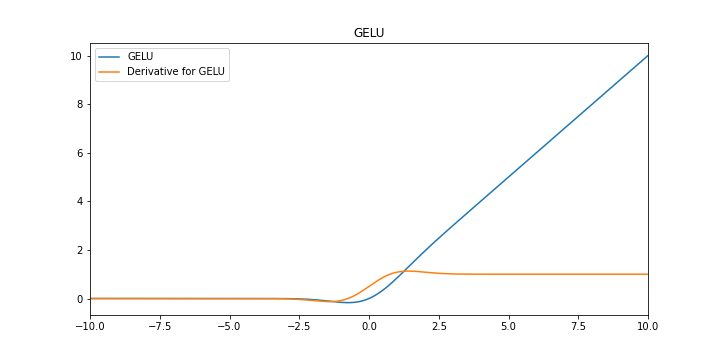
\includegraphics[width=\linewidth]{./imgs/GELU.png}


% Truely softmax = argmax


(d)
The four types of linear transformations are: dilations, shears, rotations, reflections and projections.

What is the role of linear transformation and non linear transformation in a neural network?

(e)

When we increasing the batch size, the learning rate should be decreased.
When we decrease the batch size, the learning rate should be increased.

